\documentclass[10pt]{beamer}
\usetheme{metropolis}

% ── Packages ──
\usepackage{amsmath,amssymb,amsthm}
\usepackage{tikz}
\usetikzlibrary{positioning,arrows.meta,fit,matrix,backgrounds,calc,shapes.geometric}
\usepackage{graphicx}
\usepackage{array}
\usepackage{etoolbox}

% ── Theorem environments ──
\theoremstyle{definition}
\newtheorem{defi}{Definition}[section]
\newtheorem{prop}{Proposition}[section]
\newtheorem{thm}{Theorem}[section]
\newtheorem{cor}{Corollary}[section]

% Custom theorem styles with colors
\setbeamercolor{block title}{bg=red!75!black,fg=white}
\setbeamercolor{block body}{bg=yellow!10!white}

% Proposition uses yellow title
\AtBeginEnvironment{prop}{%
  \setbeamercolor{block title}{bg=yellow!75!black,fg=black}%
  \setbeamercolor{block body}{bg=yellow!10!white}%
}
\AtEndEnvironment{prop}{%
  \setbeamercolor{block title}{bg=red!75!black,fg=white}%
}

% Theorem uses yellow title
\AtBeginEnvironment{thm}{%
  \setbeamercolor{block title}{bg=yellow!75!black,fg=black}%
  \setbeamercolor{block body}{bg=yellow!10!white}%
}
\AtEndEnvironment{thm}{%
  \setbeamercolor{block title}{bg=red!75!black,fg=white}%
}

% ── Emoji definitions ──
\newcommand{\bean}{
\includegraphics[scale=0.07]{Pictures/bean.png}}
\newcommand{\leaf}{
\includegraphics[scale=0.08]{Pictures/leaf.png}}
\newcommand{\lemon}{
\includegraphics[scale=0.08]{Pictures/lemon.png}}
\newcommand{\cow}{
\includegraphics[scale=0.08]{Pictures/cow.png}}
\newcommand{\milk}{
\includegraphics[scale=0.08]{Pictures/milk.png}}
\newcommand{\coffee}{
\includegraphics[scale=0.08]{Pictures/coffee.png}}
\newcommand{\tea}{
\includegraphics[scale=0.08]{Pictures/tea.png}}
\newcommand{\bento}{
\includegraphics[scale=0.08]{Pictures/bento.png}}
\newcommand{\ramen}{\includegraphics[scale=0.08]{Pictures/ramen.png}}
\newcommand{\cola}{
\includegraphics[scale=0.08]{Pictures/cola.png}}

% ── Highlighting ──
\newcommand{\x}[1]{\alert{\textbf{#1}}}

\title{Lecture 6: Four Fundamental Subspaces}
\subtitle{MATH203 Applied Linear Algebra}
\date{}

\begin{document}
\maketitle

% ═══════════════════════════════════════
% §0 MOTIVATION
% ═══════════════════════════════════════
\section{Motivation: Connecting the Subspaces}

\begin{frame}{Recall: The Preview from Lecture 5}

At the end of Lecture 5, we discovered something beautiful:

\begin{thm}[Preview]
$\text{Null}(A) \perp \text{Row}(A)$

Every vector in $\text{Null}(A)$ is orthogonal to every row of $A$.
\end{thm}

\vspace{1em}

\x{Why?} If $\mathbf{x} \in \text{Null}(A)$, then $A\mathbf{x} = \mathbf{0}$, which means:
$$\text{row}_i \cdot \mathbf{x} = 0 \quad \text{for all rows } i$$

\vspace{1em}

\x{Today's question}: Is this an isolated phenomenon, or part of a bigger picture?

\end{frame}

\begin{frame}{What We'll Discover Today}

For any matrix $A$, there are \x{four fundamental subspaces}:

\vspace{1em}

\begin{center}
\begin{tabular}{|c|c|c|}
\hline
\textbf{Subspace} & \textbf{Lives in} & \textbf{Dimension} \\
\hline
$\text{Col}(A)$ & $\mathbb{R}^m$ (codomain) & $r$ \\
$\text{Null}(A)$ & $\mathbb{R}^n$ (domain) & $n - r$ \\
$\text{Col}(A^T)$ & $\mathbb{R}^n$ (domain) & $r$ \\
$\text{Null}(A^T)$ & $\mathbb{R}^m$ (codomain) & $m - r$ \\
\hline
\end{tabular}
\end{center}

\vspace{1em}

\x{Discovery}: They pair up into \x{orthogonal complements}!

\end{frame}

\begin{frame}{Roadmap for Today}

\x{Strategy}: Build tools first, then reveal the full picture.

\vspace{1em}

\textbf{Part 1}: How do subspaces behave under matrix products? ($AB$)

\vspace{0.5em}

\textbf{Part 2}: What is transpose? (Flipping the ingredient table)

\vspace{0.5em}

\textbf{Part 3}: The four fundamental subspaces and their orthogonality

\vspace{0.5em}

\textbf{Part 4}: Dimension relationships

\vspace{1em}

\x{Goal}: Understand the complete geometric structure of a matrix.

\end{frame}

% ═══════════════════════════════════════
% §1 SUBSPACES OF MATRIX PRODUCTS
% ═══════════════════════════════════════
\section{Subspaces of Matrix Products}

\begin{frame}{Setup: Two-Stage Production}

Imagine a \x{two-stage coffee shop}:

\vspace{1em}

\begin{center}
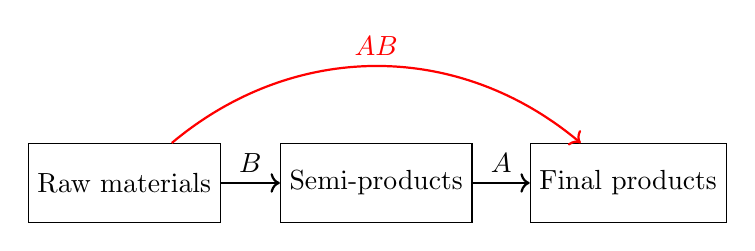
\begin{tikzpicture}[scale=0.8]
\node[draw, rectangle, minimum width=2cm, minimum height=1cm] (raw) at (0,0) {Raw materials};
\node[draw, rectangle, minimum width=2cm, minimum height=1cm] (semi) at (4,0) {Semi-products};
\node[draw, rectangle, minimum width=2cm, minimum height=1cm] (final) at (8,0) {Final products};

\draw[->, thick] (raw) -- node[above] {$B$} (semi);
\draw[->, thick] (semi) -- node[above] {$A$} (final);
\draw[->, thick, red, bend left=40] (raw) to node[above] {$AB$} (final);
\end{tikzpicture}
\end{center}

\vspace{1em}

\begin{itemize}
\item $B$: raw materials $\to$ semi-products (e.g., roasted beans, brewed tea)
\item $A$: semi-products $\to$ final products (e.g., latte, bubble tea)
\item $AB$: raw materials $\to$ final products (combined process)
\end{itemize}

\vspace{1em}

\x{Question}: How do the column spaces and null spaces of $A$, $B$, and $AB$ relate?

\end{frame}

\begin{frame}[fragile]{Concrete Example: Two Matrices}

Let's use actual matrices:

\vspace{1em}

$$B = \begin{pmatrix} 1 & 0 & 2 \\ 0 & 1 & 1 \\ 0 & 0 & 0 \end{pmatrix} \quad (3 \times 3)$$

$$A = \begin{pmatrix} 2 & 1 & 0 \\ 1 & 0 & 0 \end{pmatrix} \quad (2 \times 3)$$

\vspace{1em}

\x{Product} $AB$:

$$AB = \begin{pmatrix} 2 & 1 & 0 \\ 1 & 0 & 0 \end{pmatrix} \begin{pmatrix} 1 & 0 & 2 \\ 0 & 1 & 1 \\ 0 & 0 & 0 \end{pmatrix} = \begin{pmatrix} 2 & 1 & 5 \\ 1 & 0 & 2 \end{pmatrix}$$

\vspace{1em}

We'll investigate: What are $\text{Col}(A)$, $\text{Col}(B)$, $\text{Col}(AB)$?

\end{frame}

\begin{frame}{Visual: Column Space Containment}

\x{Key observation}: Every column of $AB$ is built from columns of $A$.

\vspace{1em}

\begin{center}
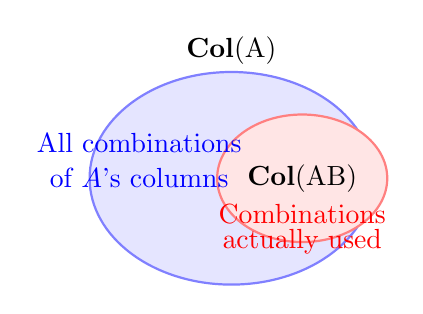
\begin{tikzpicture}[scale=0.9]
% Draw three sets
\draw[thick, blue!50, fill=blue!10] (0,0) ellipse (2cm and 1.5cm);
\draw[thick, red!50, fill=red!10] (1,0) ellipse (1.2cm and 0.9cm);

\node at (0, 1.8) {\textbf{Col}(A)};
\node at (1, 0) {\textbf{Col}(AB)};

\node[blue] at (-1.3, 0.5) {All combinations};
\node[blue] at (-1.3, 0) {of $A$'s columns};

\node[red] at (1, -0.5) {Combinations};
\node[red] at (1, -0.9) {actually used};
\end{tikzpicture}
\end{center}

\vspace{0.5em}

\x{Why?} Column $j$ of $AB$ equals $A$ times column $j$ of $B$.

So every column of $AB$ is a \x{linear combination of $A$'s columns}.

\end{frame}

\begin{frame}{Theorem 1: Column Space of Product}

\begin{thm}
$\text{Col}(AB) \subseteq \text{Col}(A)$

The column space of $AB$ is always contained in the column space of $A$.
\end{thm}

\vspace{1em}

\x{Proof}:

Write $B$ with columns $\mathbf{b}_1, \ldots, \mathbf{b}_n$:
$$B = \begin{pmatrix} | & | & & | \\ \mathbf{b}_1 & \mathbf{b}_2 & \cdots & \mathbf{b}_n \\ | & | & & | \end{pmatrix}$$

Then $AB$ has columns:
$$AB = \begin{pmatrix} | & | & & | \\ A\mathbf{b}_1 & A\mathbf{b}_2 & \cdots & A\mathbf{b}_n \\ | & | & & | \end{pmatrix}$$

Each $A\mathbf{b}_j$ is a linear combination of $A$'s columns. \qed

\end{frame}

\begin{frame}{Why This Makes Sense: Column View of Matrix Product}

Recall from Lecture 1: column $j$ of $AB$ equals $A \cdot$ (column $j$ of $B$).

\vspace{1em}

\x{Example}: If $\mathbf{b}_j = \begin{pmatrix} 2 \\ -1 \\ 3 \end{pmatrix}$ and $A$ has columns $\mathbf{a}_1, \mathbf{a}_2, \mathbf{a}_3$:

$$A\mathbf{b}_j = 2\mathbf{a}_1 - 1\mathbf{a}_2 + 3\mathbf{a}_3$$

\vspace{1em}

This is a \x{recipe} using $A$'s columns as ingredients!

\vspace{1em}

\x{Conclusion}: Every column of $AB$ is cooked from $A$'s columns.

Therefore $\text{Col}(AB) \subseteq \text{Col}(A)$.

\end{frame}

\begin{frame}{Verify with Our Example}

$$A = \begin{pmatrix} 2 & 1 & 0 \\ 1 & 0 & 0 \end{pmatrix}, \quad AB = \begin{pmatrix} 2 & 1 & 5 \\ 1 & 0 & 2 \end{pmatrix}$$

\x{Column space of $AB$}:
$$\text{Col}(AB) = \text{span}\left\{\begin{pmatrix} 2\\1 \end{pmatrix}, \begin{pmatrix} 1\\0 \end{pmatrix}, \begin{pmatrix} 5\\2 \end{pmatrix}\right\}$$

Notice: $\begin{pmatrix} 5\\2 \end{pmatrix} = 2\begin{pmatrix} 2\\1 \end{pmatrix} + 1\begin{pmatrix} 1\\0 \end{pmatrix}$ (dependent!)

So actually: $\text{Col}(AB) = \text{span}\left\{\begin{pmatrix} 2\\1 \end{pmatrix}, \begin{pmatrix} 1\\0 \end{pmatrix}\right\} = \mathbb{R}^2$

\x{Column space of $A$}:
$$\text{Col}(A) = \text{span}\left\{\begin{pmatrix} 2\\1 \end{pmatrix}, \begin{pmatrix} 1\\0 \end{pmatrix}\right\} = \mathbb{R}^2$$

Indeed: $\text{Col}(AB) \subseteq \text{Col}(A)$ \checkmark \quad (Equality in this case!)

\end{frame}

\begin{frame}{Theorem 2: Null Space Inclusion}

\begin{thm}
$\text{Null}(B) \subseteq \text{Null}(AB)$

The null space of $B$ is always contained in the null space of $AB$.
\end{thm}

\vspace{1em}

\x{Proof}:

If $\mathbf{x} \in \text{Null}(B)$, then $B\mathbf{x} = \mathbf{0}$.

Therefore:
$$(AB)\mathbf{x} = A(B\mathbf{x}) = A(\mathbf{0}) = \mathbf{0}$$

So $\mathbf{x} \in \text{Null}(AB)$. \qed

\end{frame}

\begin{frame}{Why This Makes Sense: Linear Dependencies Persist}

Recall from Lecture 5: $\mathbf{x} \in \text{Null}(B)$ records a \x{linear dependence} among columns of $B$.

\vspace{1em}

\x{Example}: If $\mathbf{x} = \begin{pmatrix} 2 \\ -1 \\ 0 \end{pmatrix} \in \text{Null}(B)$, this says:
$$2\mathbf{b}_1 - 1\mathbf{b}_2 + 0\mathbf{b}_3 = \mathbf{0}$$

\vspace{1em}

\x{What happens when we apply $A$ to both sides?}
$$A(2\mathbf{b}_1 - 1\mathbf{b}_2) = 2(A\mathbf{b}_1) - 1(A\mathbf{b}_2) = 2(AB)_1 - 1(AB)_2 = \mathbf{0}$$

\vspace{1em}

\x{Conclusion}: The \x{same linear dependence} holds for columns of $AB$!

\vspace{0.5em}

Applying $A$ preserves all existing linear relations.

\end{frame}

\begin{frame}{Verify with Our Example}

$$B = \begin{pmatrix} 1 & 0 & 2 \\ 0 & 1 & 1 \\ 0 & 0 & 0 \end{pmatrix}$$

\vspace{1em}

\x{Find $\text{Null}(B)$}:

By inspection, column 3 of $B$ equals $2 \times$ column 1 plus $1 \times$ column 2:
$$\begin{pmatrix} 2\\1\\0 \end{pmatrix} = 2\begin{pmatrix} 1\\0\\0 \end{pmatrix} + 1\begin{pmatrix} 0\\1\\0 \end{pmatrix}$$

So the dependence relation is: $-2\mathbf{b}_1 - 1\mathbf{b}_2 + 1\mathbf{b}_3 = \mathbf{0}$

$$\text{Null}(B) = \text{span}\left\{\begin{pmatrix} -2\\-1\\1 \end{pmatrix}\right\}$$

\end{frame}

\begin{frame}{Verify with Our Example (continued)}

$$AB = \begin{pmatrix} 2 & 1 & 5 \\ 1 & 0 & 2 \end{pmatrix}$$

\x{Check}: Does $\begin{pmatrix} -2\\-1\\1 \end{pmatrix} \in \text{Null}(AB)$?

$$AB\begin{pmatrix} -2\\-1\\1 \end{pmatrix} = \begin{pmatrix} 2 & 1 & 5 \\ 1 & 0 & 2 \end{pmatrix}\begin{pmatrix} -2\\-1\\1 \end{pmatrix} = \begin{pmatrix} -4-1+5\\-2+0+2 \end{pmatrix} = \begin{pmatrix} 0\\0 \end{pmatrix}$$

Yes! \checkmark

\x{Find $\text{Null}(AB)$ completely}:

Column 3 of $AB$ equals $2 \times$ column 1 plus $1 \times$ column 2:
$$\text{Null}(AB) = \text{span}\left\{\begin{pmatrix} -2\\-1\\1 \end{pmatrix}\right\}$$

So $\text{Null}(AB) = \text{Null}(B)$ (equality!) in this example.

\end{frame}

\begin{frame}{The Big Question}

We've seen:

\begin{itemize}
\item $\text{Col}(AB) \subseteq \text{Col}(A)$ (always)
\item $\text{Null}(B) \subseteq \text{Null}(AB)$ (always)
\end{itemize}

\x{But}: In our example, we had \x{equality} in both cases!

\begin{center}
\Large
\textbf{When is $\text{Null}(AB) = \text{Null}(B)$ exactly?}
\end{center}

\x{Meaning}: When does multiplication by $A$ \x{not create new dependencies}?

\end{frame}

\begin{frame}{Theorem 3: The Equivalence}

\begin{thm}
$$\text{Null}(A) \cap \text{Col}(B) = \{\mathbf{0}\} \quad \Longleftrightarrow \quad \text{Null}(AB) = \text{Null}(B)$$
\end{thm}

\vspace{1em}

\x{Left side}: Among all vectors $B$ can produce, none (except $\mathbf{0}$) lands in $\text{Null}(A)$.

\vspace{1em}

\x{Right side}: All dependencies in $AB$ were already in $B$ (no new ones created).

\vspace{1em}

These are \x{two perspectives on the same phenomenon}!

\end{frame}

\begin{frame}[fragile]{Visual: The Equivalence}

\begin{center}
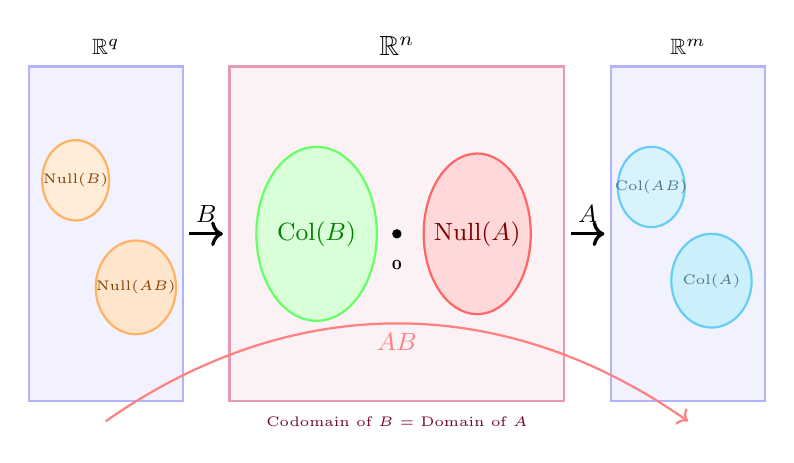
\begin{tikzpicture}[scale=0.85]
% Left: Domain of B (R^q)
\draw[thick, blue!30, fill=blue!5] (-2.5,-2.5) rectangle (-0.2,2.5);
\node at (-1.35, 2.8) {\footnotesize $\mathbb{R}^q$};

% Null(B) in left space
\draw[thick, orange!60, fill=orange!15] (-1.8, 0.8) ellipse (0.5cm and 0.6cm);
\node[orange!50!black, font=\tiny] at (-1.8, 0.8) {Null$(B)$};

% Null(AB) in left space
\draw[thick, orange!60, fill=orange!20] (-0.9, -0.8) ellipse (0.6cm and 0.7cm);
\node[orange!50!black, font=\tiny] at (-0.9, -0.8) {Null$(AB)$};

% Middle: Codomain of B = Domain of A (R^n)
\draw[thick, purple!40, fill=purple!5] (0.5,-2.5) rectangle (5.5,2.5);
\node at (3, 2.8) {\textbf{$\mathbb{R}^n$}};
\node[purple!60!black, font=\tiny] at (3, -2.8) {Codomain of $B$ = Domain of $A$};

% Col(B) in the middle space
\draw[thick, green!60, fill=green!15] (1.8, 0) ellipse (0.9cm and 1.3cm);
\node[green!50!black, font=\small] at (1.8, 0) {Col$(B)$};

% Null(A) in the middle space
\draw[thick, red!60, fill=red!15] (4.2, 0) ellipse (0.8cm and 1.2cm);
\node[red!50!black, font=\small] at (4.2, 0) {Null$(A)$};

% Zero vector at intersection
\fill (3, 0) circle (2pt);
\node[below, font=\tiny] at (3, -0.25) {$\mathbf{0}$};

% Right: Codomain of A (R^m)
\draw[thick, blue!30, fill=blue!5] (6.2,-2.5) rectangle (8.5,2.5);
\node at (7.35, 2.8) {\footnotesize $\mathbb{R}^m$};

% Col(AB) in right space
\draw[thick, cyan!60, fill=cyan!15] (6.8, 0.7) ellipse (0.5cm and 0.6cm);
\node[cyan!50!black, font=\tiny] at (6.8, 0.7) {Col$(AB)$};

% Col(A) in right space
\draw[thick, cyan!60, fill=cyan!20] (7.7, -0.7) ellipse (0.6cm and 0.7cm);
\node[cyan!50!black, font=\tiny] at (7.7, -0.7) {Col$(A)$};

% Arrows
\draw[->, very thick] (-0.1, 0) -- node[above, font=\small] {$B$} (0.4, 0);
\draw[->, very thick] (5.6, 0) -- node[above, font=\small] {$A$} (6.1, 0);

% Composition arrow
\draw[->, thick, red!50, bend left=35] (-1.35, -2.8) to node[below, font=\small] {$AB$} (7.35, -2.8);
\end{tikzpicture}
\end{center}

\vspace{-0.3em}

\x{Key}: Col$(B)$ and Null$(A)$ both live in $\mathbb{R}^n$. Do they intersect?

If \x{only at $\mathbf{0}$}: Null$(AB) =$ Null$(B)$ (no new dependencies created)

\end{frame}

\begin{frame}{Proof Direction (a): $\Rightarrow$}

\x{Assume}: $\text{Null}(A) \cap \text{Col}(B) = \{\mathbf{0}\}$

\x{Goal}: Show $\text{Null}(AB) = \text{Null}(B)$

\vspace{1em}

We already know $\text{Null}(B) \subseteq \text{Null}(AB)$ (Theorem 2).

To show equality, prove the reverse inclusion.

\vspace{1em}

Take any $\mathbf{x} \in \text{Null}(AB)$. Then $(AB)\mathbf{x} = \mathbf{0}$, so:
$$A(B\mathbf{x}) = \mathbf{0}$$

This means $B\mathbf{x} \in \text{Null}(A)$.

\end{frame}

\begin{frame}{Proof Direction (a): $\Rightarrow$ (continued)}

We have: $B\mathbf{x} \in \text{Null}(A)$.

\vspace{1em}

But also: $B\mathbf{x} \in \text{Col}(B)$ (by definition of column space).

\vspace{1em}

Therefore: $B\mathbf{x} \in \text{Null}(A) \cap \text{Col}(B)$.

\vspace{1em}

By assumption, $\text{Null}(A) \cap \text{Col}(B) = \{\mathbf{0}\}$, so:
$$B\mathbf{x} = \mathbf{0}$$

\vspace{1em}

This means $\mathbf{x} \in \text{Null}(B)$.

\vspace{1em}

We've shown $\text{Null}(AB) \subseteq \text{Null}(B)$. Combined with Theorem 2:
$$\text{Null}(AB) = \text{Null}(B)$$ \qed

\end{frame}

\begin{frame}{Proof Direction (b): $\Leftarrow$}

\x{Assume}: $\text{Null}(AB) = \text{Null}(B)$

\x{Goal}: Show $\text{Null}(A) \cap \text{Col}(B) = \{\mathbf{0}\}$

\vspace{1em}

Suppose $\mathbf{v} \in \text{Null}(A) \cap \text{Col}(B)$.

\vspace{1em}

Since $\mathbf{v} \in \text{Null}(A)$: $A\mathbf{v} = \mathbf{0}$.

Since $\mathbf{v} \in \text{Col}(B)$: $\mathbf{v} = B\mathbf{x}$ for some $\mathbf{x}$.

\vspace{1em}

Combining:
$$A(B\mathbf{x}) = A\mathbf{v} = \mathbf{0}$$

So $(AB)\mathbf{x} = \mathbf{0}$, meaning $\mathbf{x} \in \text{Null}(AB)$.

\end{frame}

\begin{frame}{Proof Direction (b): $\Leftarrow$ (continued)}

We have: $\mathbf{x} \in \text{Null}(AB)$.

\vspace{1em}

By hypothesis, $\text{Null}(AB) = \text{Null}(B)$, so:
$$\mathbf{x} \in \text{Null}(B)$$

\vspace{1em}

Therefore:
$$B\mathbf{x} = \mathbf{0}$$

\vspace{1em}

But we had $\mathbf{v} = B\mathbf{x}$, so:
$$\mathbf{v} = \mathbf{0}$$

\vspace{1em}

We've shown: any $\mathbf{v} \in \text{Null}(A) \cap \text{Col}(B)$ must be $\mathbf{0}$.

Therefore: $\text{Null}(A) \cap \text{Col}(B) = \{\mathbf{0}\}$ \qed

\end{frame}

\begin{frame}{Summary: Subspaces of Matrix Products}

\begin{center}
\begin{tabular}{|l|l|}
\hline
\textbf{Theorem} & \textbf{Meaning} \\
\hline
$\text{Col}(AB) \subseteq \text{Col}(A)$ & Columns of $AB$ built from $A$'s columns \\
& \\
$\text{Null}(B) \subseteq \text{Null}(AB)$ & Dependencies in $B$ persist in $AB$ \\
& \\
$\text{Null}(A) \cap \text{Col}(B) = \{\mathbf{0}\}$ & No new dependencies created \\
$\Leftrightarrow$ & \\
$\text{Null}(AB) = \text{Null}(B)$ & \\
\hline
\end{tabular}
\end{center}

\vspace{1em}

\x{Key insight}: Matrix multiplication has predictable effects on subspaces.

\vspace{0.5em}

\x{Next}: We need a new tool to reveal deeper relationships — \x{transpose}.

\end{frame}

% ═══════════════════════════════════════
% §2 TRANSPOSE
% ═══════════════════════════════════════
\section{Transpose: Flipping the Production Table}

\begin{frame}{What Is Transpose? Flipping Perspective}

In our ingredient table framework:

\vspace{1em}

\begin{itemize}
\item \x{Rows} = raw materials (inputs)
\item \x{Columns} = products (outputs)
\item \x{Entry $A_{ij}$} = amount of material $i$ needed for product $j$
\end{itemize}

\vspace{1em}

\x{Original question}: Given a product, how much of each material do we need?

\vspace{1em}

\x{Flipped question}: Given a material, which products use it?

\vspace{1em}

This perspective flip is called \x{transpose}.

\end{frame}

\begin{frame}{Concrete Example: Coffee Shop Ingredient Table}

\x{Original table $A$} (materials $\to$ products):

\vspace{0.5em}

\begin{center}
\begin{tabular}{c|ccc}
 & \milk & \coffee & \tea \\
\hline
\leaf & 0 & 0 & 2 \\
\lemon & 0 & 0 & 1 \\
\bean & 0 & 2 & 4 \\
\cow & 1 & 0 & 1
\end{tabular}
$\quad = \begin{pmatrix} 0 & 0 & 2 \\ 0 & 0 & 1 \\ 0 & 2 & 4 \\ 1 & 0 & 1 \end{pmatrix}$
\end{center}

\vspace{0.5em}

\x{Reading}:
\begin{itemize}
\item Column \milk: needs $(0\text{\leaf}, 0\text{\lemon}, 0\text{\bean}, 1\text{\cow})$
\item Row \leaf: distributed to products as $(0, 0, 2)$
\end{itemize}

\end{frame}

\begin{frame}{Flipped Table: Transpose $A^T$}

\x{Flipped table $A^T$} (products $\to$ materials):

\vspace{0.5em}

\begin{center}
\begin{tabular}{c|cccc}
 & \leaf & \lemon & \bean & \cow \\
\hline
\milk & 0 & 0 & 0 & 1 \\
\coffee & 0 & 0 & 2 & 0 \\
\tea & 2 & 1 & 4 & 1
\end{tabular}
$\quad = \begin{pmatrix} 0 & 0 & 0 & 1 \\ 0 & 0 & 2 & 0 \\ 2 & 1 & 4 & 1 \end{pmatrix}$
\end{center}

\vspace{0.5em}

\x{Reading}:
\begin{itemize}
\item Row \milk: contains amounts $(0\text{\leaf}, 0\text{\lemon}, 0\text{\bean}, 1\text{\cow})$
\item Column \leaf: contributes to products as $(0, 0, 2)$
\end{itemize}

\vspace{1em}

\x{Notice}: Rows of $A$ become columns of $A^T$, and vice versa!

\end{frame}

\begin{frame}[fragile]{Visual: Flipping the Table}

\begin{center}
\begin{tikzpicture}[scale=0.9]
% Original matrix A
\matrix (A) [matrix of math nodes, left delimiter=(, right delimiter=),
             nodes={minimum width=1em, minimum height=1.2em}] at (0,0) {
0 & 0 & 2 \\
0 & 0 & 1 \\
0 & 2 & 4 \\
1 & 0 & 1 \\
};

% Labels for A
\node[left=0.3cm of A-1-1] {\tiny \leaf};
\node[left=0.3cm of A-2-1] {\tiny \lemon};
\node[left=0.3cm of A-3-1] {\tiny \bean};
\node[left=0.3cm of A-4-1] {\tiny \cow};
\node[above=0.2cm of A-1-1] {\tiny \milk};
\node[above=0.2cm of A-1-2] {\tiny \coffee};
\node[above=0.2cm of A-1-3] {\tiny \tea};

\node[below=0.5cm of A] {$A$ (materials = rows)};

% Arrow
\draw[->, ultra thick, red] (3, 0) -- node[above] {Flip} (5, 0);

% Transposed matrix A^T
\matrix (AT) [matrix of math nodes, left delimiter=(, right delimiter=),
              nodes={minimum width=1em, minimum height=1.2em}] at (8,0) {
0 & 0 & 0 & 1 \\
0 & 0 & 2 & 0 \\
2 & 1 & 4 & 1 \\
};

% Labels for A^T
\node[left=0.3cm of AT-1-1] {\tiny \milk};
\node[left=0.3cm of AT-2-1] {\tiny \coffee};
\node[left=0.3cm of AT-3-1] {\tiny \tea};
\node[above=0.2cm of AT-1-1] {\tiny \leaf};
\node[above=0.2cm of AT-1-2] {\tiny \lemon};
\node[above=0.2cm of AT-1-3] {\tiny \bean};
\node[above=0.2cm of AT-1-4] {\tiny \cow};

\node[below=0.5cm of AT] {$A^T$ (products = rows)};
\end{tikzpicture}
\end{center}

\vspace{0.5em}

\x{Key}: The rows and columns swap roles!

\end{frame}

\begin{frame}{Formal Definition}

\begin{defi}[Transpose]
For an $m \times n$ matrix $A$, its \x{transpose} $A^T$ is the $n \times m$ matrix:
$$(A^T)_{ij} = A_{ji}$$

Rows of $A$ become columns of $A^T$, and columns of $A$ become rows of $A^T$.
\end{defi}

\vspace{1em}

\x{Example}:
$$A = \begin{pmatrix} 1 & 2 & 3 \\ 4 & 5 & 6 \end{pmatrix} \quad \Rightarrow \quad A^T = \begin{pmatrix} 1 & 4 \\ 2 & 5 \\ 3 & 6 \end{pmatrix}$$

\vspace{1em}

Row 1 of $A$: $(1, 2, 3)$ becomes column 1 of $A^T$: $\begin{pmatrix} 1\\2\\3 \end{pmatrix}$

\end{frame}

\begin{frame}{Property 1: Transpose of Product}

\begin{prop}
$$(AB)^T = B^T A^T$$

The transpose of a product reverses the order!
\end{prop}

\vspace{1em}

\x{Proof} (entry-by-entry):

Entry $(i,j)$ of $(AB)^T$:
$$(AB)^T_{ij} = (AB)_{ji} = \sum_k A_{jk} B_{ki}$$

Entry $(i,j)$ of $B^T A^T$:
$$(B^T A^T)_{ij} = \sum_k (B^T)_{ik} (A^T)_{kj} = \sum_k B_{ki} A_{jk}$$

Since multiplication of numbers commutes: $\sum_k A_{jk} B_{ki} = \sum_k B_{ki} A_{jk}$ \qed

\end{frame}

\begin{frame}{Why the Order Reverses: Production View}

In a two-stage production $A \cdot B$:

\vspace{0.5em}

\begin{itemize}
\item $B$: raw materials $\to$ semi-products
\item $A$: semi-products $\to$ final products
\end{itemize}

\vspace{1em}

\x{Forward direction} ($AB$): raw $\xrightarrow{B}$ semi $\xrightarrow{A}$ final

\vspace{1em}

\x{Flipped perspective} (transpose):
\begin{itemize}
\item $A^T$: final product $\to$ which semi-products it uses
\item $B^T$: semi-product $\to$ which raw materials it needs
\end{itemize}

\vspace{1em}

\x{Backward tracing}: final $\xrightarrow{A^T}$ semi $\xrightarrow{B^T}$ raw

\vspace{1em}

Hence $(AB)^T = B^T A^T$ — the order flips!

\end{frame}

\begin{frame}{Property 2: Transpose of Inverse}

\begin{prop}
If $A$ is invertible:
$$(A^{-1})^T = (A^T)^{-1}$$

Transpose and inverse commute.
\end{prop}

\vspace{1em}

\x{Proof}:

Start from $A \cdot A^{-1} = I$, transpose both sides:
$$(A \cdot A^{-1})^T = I^T = I$$

Using Property 1:
$$(A^{-1})^T \cdot A^T = I$$

Similarly, $(A^{-1} \cdot A)^T = I$ gives $A^T \cdot (A^{-1})^T = I$.

Therefore $(A^{-1})^T$ is the inverse of $A^T$. \qed

\end{frame}

\begin{frame}{Property 3: Transpose is Linear}

\begin{prop}
$$(A + B)^T = A^T + B^T$$

Transpose distributes over addition.
\end{prop}

\vspace{1em}

\x{Proof} (entry-by-entry):
\begin{align*}
(A + B)^T_{ij} &= (A + B)_{ji} \\
&= A_{ji} + B_{ji} \\
&= (A^T)_{ij} + (B^T)_{ij} \\
&= (A^T + B^T)_{ij}
\end{align*}

Therefore $(A + B)^T = A^T + B^T$. \qed

\end{frame}

\begin{frame}{Symmetric Matrices}

\begin{defi}[Symmetric Matrix]
A matrix $S$ is \x{symmetric} if $S^T = S$.

The ingredient table looks the same when flipped!
\end{defi}

\vspace{1em}

\x{Example}:
$$S = \begin{pmatrix} 1 & 2 & 3 \\ 2 & 4 & 5 \\ 3 & 5 & 6 \end{pmatrix}$$

Flipping rows $\leftrightarrow$ columns gives the same matrix.

\vspace{1em}

\x{Notice}: $S_{ij} = S_{ji}$ for all $i, j$ (mirror symmetry across diagonal).

\end{frame}

\begin{frame}{Theorem: $AA^T$ and $A^T A$ Are Always Symmetric}

\begin{thm}
For any matrix $A$:
\begin{enumerate}
\item $AA^T$ is symmetric
\item $A^T A$ is symmetric
\end{enumerate}
\end{thm}

\vspace{1em}

\x{Proof}:

Using $(AB)^T = B^T A^T$:

$$(AA^T)^T = (A^T)^T A^T = A A^T$$

So $AA^T$ is symmetric.

\vspace{1em}

Similarly:
$$(A^T A)^T = A^T (A^T)^T = A^T A$$

So $A^T A$ is symmetric. \qed

\end{frame}

\begin{frame}{Verify with Concrete Matrix}

$$A = \begin{pmatrix} 1 & 2 \\ 3 & 4 \\ 5 & 6 \end{pmatrix}, \quad A^T = \begin{pmatrix} 1 & 3 & 5 \\ 2 & 4 & 6 \end{pmatrix}$$

\vspace{1em}

\x{Compute $AA^T$}:

$$AA^T = \begin{pmatrix} 1 & 2 \\ 3 & 4 \\ 5 & 6 \end{pmatrix} \begin{pmatrix} 1 & 3 & 5 \\ 2 & 4 & 6 \end{pmatrix} = \begin{pmatrix} 5 & 11 & 17 \\ 11 & 25 & 39 \\ 17 & 39 & 61 \end{pmatrix}$$

Check: $(AA^T)^T = AA^T$ \checkmark \quad (symmetric!)

\end{frame}

\begin{frame}{Verify with Concrete Matrix (continued)}

$$A = \begin{pmatrix} 1 & 2 \\ 3 & 4 \\ 5 & 6 \end{pmatrix}, \quad A^T = \begin{pmatrix} 1 & 3 & 5 \\ 2 & 4 & 6 \end{pmatrix}$$

\vspace{1em}

\x{Compute $A^T A$}:

$$A^T A = \begin{pmatrix} 1 & 3 & 5 \\ 2 & 4 & 6 \end{pmatrix} \begin{pmatrix} 1 & 2 \\ 3 & 4 \\ 5 & 6 \end{pmatrix} = \begin{pmatrix} 35 & 44 \\ 44 & 56 \end{pmatrix}$$

Check: $(A^T A)^T = A^T A$ \checkmark \quad (symmetric!)

\end{frame}

\begin{frame}{Change of Perspective}

\textbf{What we've learned so far:}

\begin{itemize}
\item \x{Why} transpose exists: flipping the ingredient table perspective
\item \x{Why} $(AB)^T = B^T A^T$: backward tracing reverses order
\item \x{Why} $AA^T$ is symmetric: algebraic consequence of transpose properties
\end{itemize}

\begin{alertblock}{From This Point Forward}
We \x{forget about coffee shops} and work with abstract matrices $A$, $B$, $C$.

The key properties: $(AB)^T = B^T A^T$, symmetry of $AA^T$ and $A^T A$.

These apply to \x{all matrices}, and we'll use them to discover deeper geometric relationships.
\end{alertblock}

\x{Next}: The four fundamental subspaces and their beautiful orthogonality.

\end{frame}

% ═══════════════════════════════════════
% §3 FOUR FUNDAMENTAL SUBSPACES
% ═══════════════════════════════════════
\section{Four Fundamental Subspaces and Orthogonality}

\begin{frame}{The Four Fundamental Subspaces}

For any $m \times n$ matrix $A$, there are \x{four fundamental subspaces}:

\vspace{1em}

\begin{center}
\begin{tabular}{|l|c|c|c|}
\hline
\textbf{Subspace} & \textbf{Definition} & \textbf{Lives in} & \textbf{Dimension} \\
\hline
$\text{Col}(A)$ & $\{A\mathbf{x}\}$ & $\mathbb{R}^m$ & $r$ \\
$\text{Null}(A)$ & $\{\mathbf{x} : A\mathbf{x} = \mathbf{0}\}$ & $\mathbb{R}^n$ & $n - r$ \\
$\text{Col}(A^T)$ & $\{A^T \mathbf{y}\}$ & $\mathbb{R}^n$ & $r$ \\
$\text{Null}(A^T)$ & $\{\mathbf{y} : A^T \mathbf{y} = \mathbf{0}\}$ & $\mathbb{R}^m$ & $m - r$ \\
\hline
\end{tabular}
\end{center}

\vspace{0.5em}

where $r = \text{rank}(A)$.

\vspace{1em}

\x{Key observations}:
\begin{itemize}
\item Two subspaces in $\mathbb{R}^n$ (domain): $\text{Null}(A)$ and $\text{Col}(A^T)$
\item Two subspaces in $\mathbb{R}^m$ (codomain): $\text{Col}(A)$ and $\text{Null}(A^T)$
\end{itemize}

\end{frame}

\begin{frame}[fragile]{Visual: Two Pairs of Subspaces}

\begin{center}
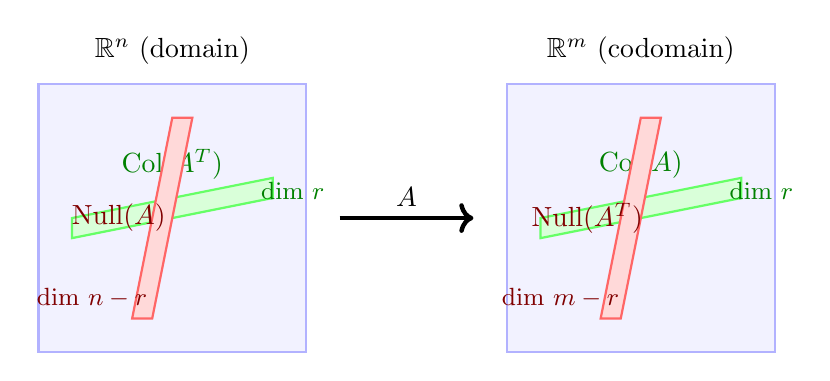
\begin{tikzpicture}[scale=0.85]
% Domain R^n
\draw[thick, blue!30, fill=blue!5] (-2,-2) rectangle (2,2);
\node at (0, 2.5) {$\mathbb{R}^n$ (domain)};

% Col(A^T)
\draw[thick, green!60, fill=green!15] (-1.5, -0.3) -- (1.5, 0.3) -- (1.5, 0.6) -- (-1.5, 0) -- cycle;
\node[green!50!black] at (0, 0.8) {Col$(A^T)$};
\node[green!50!black, font=\small] at (1.8, 0.4) {dim $r$};

% Null(A)
\draw[thick, red!60, fill=red!15] (-0.3, -1.5) -- (0.3, 1.5) -- (0, 1.5) -- (-0.6, -1.5) -- cycle;
\node[red!50!black] at (-0.8, 0) {Null$(A)$};
\node[red!50!black, font=\small] at (-1.2, -1.2) {dim $n-r$};

% Codomain R^m
\draw[thick, blue!30, fill=blue!5] (5,-2) rectangle (9,2);
\node at (7, 2.5) {$\mathbb{R}^m$ (codomain)};

% Col(A)
\draw[thick, green!60, fill=green!15] (5.5, -0.3) -- (8.5, 0.3) -- (8.5, 0.6) -- (5.5, 0) -- cycle;
\node[green!50!black] at (7, 0.8) {Col$(A)$};
\node[green!50!black, font=\small] at (8.8, 0.4) {dim $r$};

% Null(A^T)
\draw[thick, red!60, fill=red!15] (6.7, -1.5) -- (7.3, 1.5) -- (7, 1.5) -- (6.4, -1.5) -- cycle;
\node[red!50!black] at (6.2, 0) {Null$(A^T)$};
\node[red!50!black, font=\small] at (5.8, -1.2) {dim $m-r$};

% Matrix A
\draw[->, ultra thick] (2.5, 0) -- node[above] {$A$} (4.5, 0);
\end{tikzpicture}
\end{center}

\vspace{0.5em}

\x{Today's discovery}: These pairs are \x{orthogonal} to each other!

\end{frame}

\begin{frame}{Theorem 4: Col$(A^T) \perp$ Null$(A)$}

\begin{thm}
Every vector in $\text{Col}(A^T)$ is orthogonal to every vector in $\text{Null}(A)$.

Precisely: For $\mathbf{x} \in \text{Null}(A)$ and $\mathbf{y} \in \text{Col}(A^T)$,
$$\mathbf{y}^T \mathbf{x} = 0$$
\end{thm}

\vspace{1em}

\x{Meaning}: The row space and null space are perpendicular!

\end{frame}

\begin{frame}{Proof (Inner Product View)}

Let $\mathbf{x} \in \text{Null}(A)$ and $\mathbf{y} \in \text{Col}(A^T)$.

\vspace{1em}

By definition:
\begin{itemize}
\item $\mathbf{x} \in \text{Null}(A)$ means $A\mathbf{x} = \mathbf{0}$
\item $\mathbf{y} \in \text{Col}(A^T)$ means $\mathbf{y} = A^T \mathbf{z}$ for some $\mathbf{z}$
\end{itemize}

\vspace{1em}

Compute the inner product:
\begin{align*}
\mathbf{y}^T \mathbf{x} &= (A^T \mathbf{z})^T \mathbf{x} \\
&= \mathbf{z}^T (A^T)^T \mathbf{x} \\
&= \mathbf{z}^T A \mathbf{x}
\end{align*}

Since $\mathbf{x} \in \text{Null}(A)$, we have $A\mathbf{x} = \mathbf{0}$:
$$\mathbf{z}^T A \mathbf{x} = \mathbf{z}^T \mathbf{0} = 0$$ \qed

\end{frame}

\begin{frame}{Proof (Geometric View: Rows as Normal Vectors)}

The equation $A\mathbf{x} = \mathbf{0}$ can be written row-by-row:

$$\begin{pmatrix} \text{---} \mathbf{r}_1^T \text{---} \\ \text{---} \mathbf{r}_2^T \text{---} \\ \vdots \\ \text{---} \mathbf{r}_m^T \text{---} \end{pmatrix} \mathbf{x} = \begin{pmatrix} \mathbf{r}_1^T \mathbf{x} \\ \mathbf{r}_2^T \mathbf{x} \\ \vdots \\ \mathbf{r}_m^T \mathbf{x} \end{pmatrix} = \mathbf{0}$$

\vspace{1em}

This means:
$$\mathbf{r}_1^T \mathbf{x} = 0, \quad \mathbf{r}_2^T \mathbf{x} = 0, \quad \ldots, \quad \mathbf{r}_m^T \mathbf{x} = 0$$

\vspace{1em}

\x{Interpretation}: Each row $\mathbf{r}_i$ is \x{perpendicular} to $\mathbf{x}$.

\end{frame}

\begin{frame}{Proof (Geometric View: continued)}

We have: Each row $\mathbf{r}_i$ of $A$ is perpendicular to every $\mathbf{x} \in \text{Null}(A)$.

\vspace{1em}

\x{But}: The rows of $A$ are exactly the \x{columns of $A^T$}!

$$A^T = \begin{pmatrix} | & | & & | \\ \mathbf{r}_1 & \mathbf{r}_2 & \cdots & \mathbf{r}_m \\ | & | & & | \end{pmatrix}$$

\vspace{1em}

Therefore:
$$\text{Col}(A^T) = \text{span}\{\mathbf{r}_1, \mathbf{r}_2, \ldots, \mathbf{r}_m\}$$

consists of vectors perpendicular to $\text{Null}(A)$. \qed

\end{frame}

\begin{frame}[fragile]{Visual: Orthogonality in $\mathbb{R}^n$}

\begin{center}
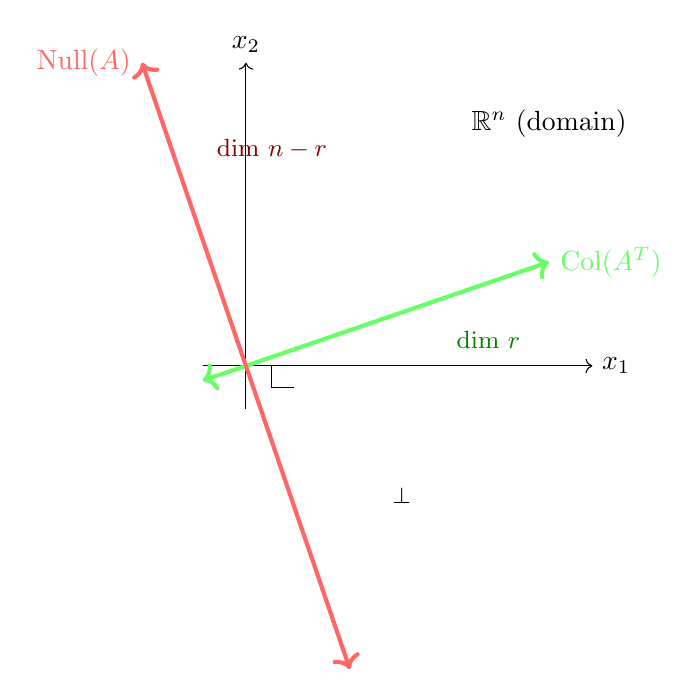
\begin{tikzpicture}[scale=1.1]
% Coordinate system
\draw[->] (-0.5,0) -- (4,0) node[right] {$x_1$};
\draw[->] (0,-0.5) -- (0,3.5) node[above] {$x_2$};

% Col(A^T) - a line through origin
\draw[thick, green!60, ->, line width=1.5pt] (0,0) -- (3.5, 1.2) node[right] {Col$(A^T)$};
\draw[thick, green!60, ->, line width=1.5pt] (0,0) -- (-0.5, -0.17);

% Null(A) - perpendicular line
\draw[thick, red!60, ->, line width=1.5pt] (0,0) -- (1.2, -3.5);
\draw[thick, red!60, ->, line width=1.5pt] (0,0) -- (-1.2, 3.5) node[left] {Null$(A)$};

% Right angle indicator
\draw (0.3, 0) -- (0.3, -0.25) -- (0.55, -0.25);

% Labels
\node at (3.5, 2.8) {$\mathbb{R}^n$ (domain)};
\node[green!50!black] at (2.8, 0.3) {\small dim $r$};
\node[red!50!black] at (0.3, 2.5) {\small dim $n-r$};

% Annotation
\node at (1.8, -1.5) {\footnotesize $\perp$};
\end{tikzpicture}
\end{center}

\vspace{0.5em}

In $\mathbb{R}^n$, the two subspaces Col$(A^T)$ and Null$(A)$ are perpendicular!

\end{frame}

\begin{frame}{Concrete Example}

$$A = \begin{pmatrix} 1 & 2 & 3 \\ 2 & 4 & 6 \end{pmatrix}$$

\x{Find Null$(A)$}:

$A\mathbf{x} = \mathbf{0}$ gives: $x_1 + 2x_2 + 3x_3 = 0$ (second row is $2 \times$ first)

Basis for Null$(A)$:
$$\text{Null}(A) = \text{span}\left\{\begin{pmatrix} -2\\1\\0 \end{pmatrix}, \begin{pmatrix} -3\\0\\1 \end{pmatrix}\right\}$$

\x{Find Col$(A^T)$}:

$$A^T = \begin{pmatrix} 1 & 2 \\ 2 & 4 \\ 3 & 6 \end{pmatrix}$$

$$\text{Col}(A^T) = \text{span}\left\{\begin{pmatrix} 1\\2\\3 \end{pmatrix}, \begin{pmatrix} 2\\4\\6 \end{pmatrix}\right\} = \text{span}\left\{\begin{pmatrix} 1\\2\\3 \end{pmatrix}\right\}$$

\end{frame}

\begin{frame}{Verify Orthogonality}

$$\text{Col}(A^T) = \text{span}\left\{\begin{pmatrix} 1\\2\\3 \end{pmatrix}\right\}, \quad \text{Null}(A) = \text{span}\left\{\begin{pmatrix} -2\\1\\0 \end{pmatrix}, \begin{pmatrix} -3\\0\\1 \end{pmatrix}\right\}$$

\x{Check orthogonality}:

$$\begin{pmatrix} 1\\2\\3 \end{pmatrix}^T \begin{pmatrix} -2\\1\\0 \end{pmatrix} = 1(-2) + 2(1) + 3(0) = 0 \quad \checkmark$$

$$\begin{pmatrix} 1\\2\\3 \end{pmatrix}^T \begin{pmatrix} -3\\0\\1 \end{pmatrix} = 1(-3) + 2(0) + 3(1) = 0 \quad \checkmark$$

Indeed, $\text{Col}(A^T) \perp \text{Null}(A)$!

\end{frame}

\begin{frame}{Theorem 5: Col$(A) \perp$ Null$(A^T)$}

\begin{thm}
Every vector in $\text{Col}(A)$ is orthogonal to every vector in $\text{Null}(A^T)$.

Precisely: For $\mathbf{x} \in \text{Col}(A)$ and $\mathbf{y} \in \text{Null}(A^T)$,
$$\mathbf{y}^T \mathbf{x} = 0$$
\end{thm}

\vspace{1em}

\x{Meaning}: The column space and left null space are perpendicular!

\end{frame}

\begin{frame}{Proof}

Let $\mathbf{y} \in \text{Null}(A^T)$ and $\mathbf{x} \in \text{Col}(A)$.

\vspace{1em}

By definition:
\begin{itemize}
\item $\mathbf{y} \in \text{Null}(A^T)$ means $A^T \mathbf{y} = \mathbf{0}$
\item $\mathbf{x} \in \text{Col}(A)$ means $\mathbf{x} = A\mathbf{z}$ for some $\mathbf{z}$
\end{itemize}

\vspace{1em}

Compute the inner product:
\begin{align*}
\mathbf{y}^T \mathbf{x} &= \mathbf{y}^T (A\mathbf{z}) \\
&= (A^T \mathbf{y})^T \mathbf{z}
\end{align*}

Since $A^T \mathbf{y} = \mathbf{0}$:
$$(A^T \mathbf{y})^T \mathbf{z} = \mathbf{0}^T \mathbf{z} = 0$$ \qed

\end{frame}

\begin{frame}{Symmetry of the Theorems}

\x{Beautiful duality}:

\vspace{1em}

\begin{itemize}
\item \textbf{Theorem 4}: $\text{Col}(A^T) \perp \text{Null}(A)$ (both in $\mathbb{R}^n$)
\item \textbf{Theorem 5}: $\text{Col}(A) \perp \text{Null}(A^T)$ (both in $\mathbb{R}^m$)
\end{itemize}

\vspace{1em}

These are \x{not two separate facts} — they're the \x{same theorem}!

\vspace{1em}

\x{Why?} Apply Theorem 4 to the matrix $A^T$ instead of $A$:
$$\text{Col}((A^T)^T) \perp \text{Null}(A^T) \quad \Rightarrow \quad \text{Col}(A) \perp \text{Null}(A^T)$$

which is exactly Theorem 5!

\vspace{1em}

\x{Deep insight}: Transpose reveals a fundamental symmetry in linear algebra.

\end{frame}

\begin{frame}{Concrete Example: The Dual Case}

Using the same matrix:
$$A = \begin{pmatrix} 1 & 2 & 3 \\ 2 & 4 & 6 \end{pmatrix}$$

\x{Find Col$(A)$}:
$$\text{Col}(A) = \text{span}\left\{\begin{pmatrix} 1\\2 \end{pmatrix}, \begin{pmatrix} 2\\4 \end{pmatrix}, \begin{pmatrix} 3\\6 \end{pmatrix}\right\} = \text{span}\left\{\begin{pmatrix} 1\\2 \end{pmatrix}\right\}$$

\x{Find Null$(A^T)$}:

$A^T \mathbf{y} = \mathbf{0}$ gives: $\begin{pmatrix} 1 & 2 \\ 2 & 4 \\ 3 & 6 \end{pmatrix} \begin{pmatrix} y_1\\y_2 \end{pmatrix} = \mathbf{0}$

All equations reduce to: $y_1 + 2y_2 = 0$

$$\text{Null}(A^T) = \text{span}\left\{\begin{pmatrix} -2\\1 \end{pmatrix}\right\}$$

\end{frame}

\begin{frame}{Concrete Example: Verify Orthogonality}

$$\text{Col}(A) = \text{span}\left\{\begin{pmatrix} 1\\2 \end{pmatrix}\right\}, \quad \text{Null}(A^T) = \text{span}\left\{\begin{pmatrix} -2\\1 \end{pmatrix}\right\}$$

\x{Check orthogonality}:

$$\begin{pmatrix} -2\\1 \end{pmatrix}^T \begin{pmatrix} 1\\2 \end{pmatrix} = (-2)(1) + (1)(2) = -2 + 2 = 0 \quad \checkmark$$

Indeed, $\text{Col}(A) \perp \text{Null}(A^T)$!

\end{frame}

\begin{frame}[fragile]{The Big Picture: Four Subspaces}

\begin{center}
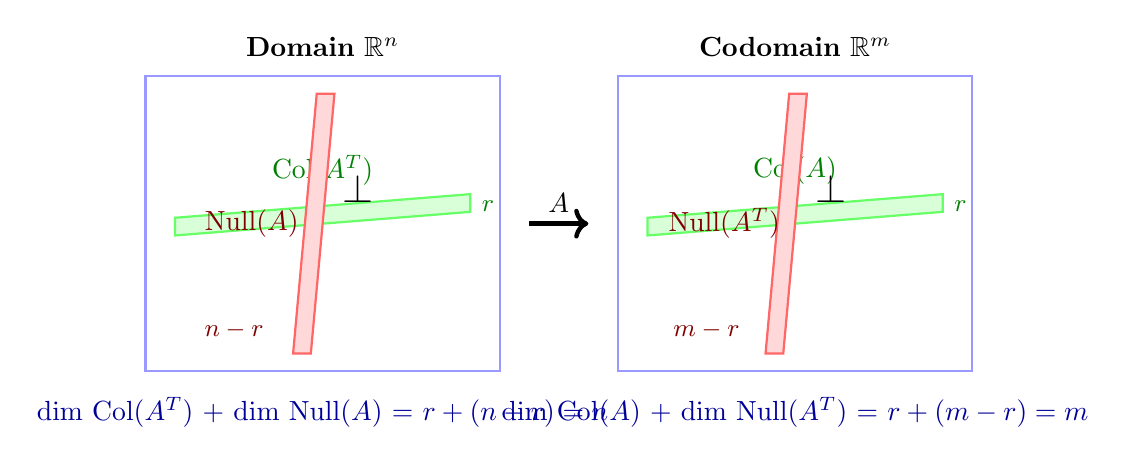
\begin{tikzpicture}[scale=0.75]
% Domain R^n box
\draw[thick, blue!40] (-3,-2.5) rectangle (3,2.5);
\node at (0, 3) {\textbf{Domain} $\mathbb{R}^n$};

% Col(A^T)
\draw[thick, green!60, fill=green!15] (-2.5, -0.2) -- (2.5, 0.2) -- (2.5, 0.5) -- (-2.5, 0.1) -- cycle;
\node[green!50!black] at (0, 0.9) {Col$(A^T)$};
\node[green!50!black, font=\small] at (2.8, 0.3) {$r$};

% Null(A)
\draw[thick, red!60, fill=red!15] (-0.2, -2.2) -- (0.2, 2.2) -- (-0.1, 2.2) -- (-0.5, -2.2) -- cycle;
\node[red!50!black] at (-1.2, 0) {Null$(A)$};
\node[red!50!black, font=\small] at (-1.5, -1.8) {$n-r$};

% Perpendicular symbol
\node at (0.6, 0.6) {\Large $\perp$};

% Codomain R^m box
\draw[thick, blue!40] (5,-2.5) rectangle (11,2.5);
\node at (8, 3) {\textbf{Codomain} $\mathbb{R}^m$};

% Col(A)
\draw[thick, green!60, fill=green!15] (5.5, -0.2) -- (10.5, 0.2) -- (10.5, 0.5) -- (5.5, 0.1) -- cycle;
\node[green!50!black] at (8, 0.9) {Col$(A)$};
\node[green!50!black, font=\small] at (10.8, 0.3) {$r$};

% Null(A^T)
\draw[thick, red!60, fill=red!15] (7.8, -2.2) -- (8.2, 2.2) -- (7.9, 2.2) -- (7.5, -2.2) -- cycle;
\node[red!50!black] at (6.8, 0) {Null$(A^T)$};
\node[red!50!black, font=\small] at (6.5, -1.8) {$m-r$};

% Perpendicular symbol
\node at (8.6, 0.6) {\Large $\perp$};

% Matrix A arrow
\draw[->, ultra thick] (3.5, 0) -- node[above] {$A$} (4.5, 0);

% Dimension totals
\node[blue!60!black] at (0, -3.2) {dim Col$(A^T)$ + dim Null$(A)$ = $r + (n-r) = n$};
\node[blue!60!black] at (8, -3.2) {dim Col$(A)$ + dim Null$(A^T)$ = $r + (m-r) = m$};
\end{tikzpicture}
\end{center}

\vspace{0.5em}

\x{Key}: The orthogonal pairs completely fill their spaces!

\end{frame}

% ═══════════════════════════════════════
% §4 DIMENSION RELATIONSHIPS
% ═══════════════════════════════════════
\section{Dimension Relationships}

\begin{frame}{Theorem 6: Row Rank Equals Column Rank}

\begin{thm}
$$\text{rank}(A) = \text{rank}(A^T)$$

The dimension of Col$(A)$ equals the dimension of Col$(A^T)$.

In other words: \x{Column rank = Row rank}.
\end{thm}

\vspace{1em}

\x{Proof idea} (using cross-filling from Lecture 3):

Any matrix can be decomposed:
$$A = R_1 + R_2 + \cdots + R_r = UV$$

where $U$ is $m \times r$ and $V$ is $r \times n$.

\end{frame}

\begin{frame}{Proof of Theorem 6 (continued)}

$$A = UV$$

where:
\begin{itemize}
\item $U$ is $m \times r$ with $r$ linearly independent columns
\item $V$ is $r \times n$ with $r$ linearly independent rows
\end{itemize}

\x{Column rank}:
$$\text{Col}(A) = \text{Col}(UV) = \text{Col}(U)$$

So dim(Col$(A)$) $= r$.

\x{Row rank}:

The rows of $A = UV$ are linear combinations of the rows of $V$.

Since $V$ has $r$ linearly independent rows, dim(Col$(A^T)$) $= r$.

Therefore $\text{rank}(A) = \text{rank}(A^T) = r$. \qed

\end{frame}

\begin{frame}{Dimension Formulas}

From the rank-nullity theorem (Lecture 5) and orthogonality:

\begin{prop}
For an $m \times n$ matrix $A$ with rank$(A) = r$:

\textbf{In $\mathbb{R}^n$ (domain):}
$$\dim(\text{Col}(A^T)) + \dim(\text{Null}(A)) = r + (n - r) = n$$

\textbf{In $\mathbb{R}^m$ (codomain):}
$$\dim(\text{Col}(A)) + \dim(\text{Null}(A^T)) = r + (m - r) = m$$
\end{prop}

\x{Meaning}: The orthogonal pairs together \x{span their entire spaces}.

\end{frame}

% ═══════════════════════════════════════
% §5 SUMMARY
% ═══════════════════════════════════════
\section{Summary}

\begin{frame}{What We Achieved Today}

\x{1. Subspaces of Matrix Products}:
\begin{itemize}
\item Col$(AB) \subseteq$ Col$(A)$ — columns of $AB$ built from $A$'s columns
\item Null$(B) \subseteq$ Null$(AB)$ — dependencies persist
\item Null$(A) \cap$ Col$(B) = \{\mathbf{0}\} \Leftrightarrow$ Null$(AB) =$ Null$(B)$ — no new dependencies
\end{itemize}

\vspace{0.5em}

\x{2. Transpose}:
\begin{itemize}
\item Flipping the ingredient table perspective
\item $(AB)^T = B^T A^T$ — order reverses
\item $AA^T$ and $A^T A$ always symmetric
\end{itemize}

\end{frame}

\begin{frame}{What We Achieved Today (continued)}

\x{3. Four Fundamental Subspaces}:
\begin{itemize}
\item Col$(A^T) \perp$ Null$(A)$ in $\mathbb{R}^n$
\item Col$(A) \perp$ Null$(A^T)$ in $\mathbb{R}^m$
\item These are dual statements — same theorem applied to $A$ and $A^T$
\end{itemize}

\vspace{0.5em}

\x{4. Dimension Relationships}:
\begin{itemize}
\item rank$(A) =$ rank$(A^T)$ — column rank equals row rank
\item dim(Col$(A^T)$) + dim(Null$(A)$) $= n$
\item dim(Col$(A)$) + dim(Null$(A^T)$) $= m$
\end{itemize}

\vspace{1em}

\x{Key insight}: The four fundamental subspaces form two orthogonal pairs that completely describe the geometry of a matrix.

\end{frame}

\begin{frame}{Preview: Next Lecture}

\x{Lecture 7}: Linear Transformations and Projections

\vspace{1em}

Now that we understand the four fundamental subspaces and their orthogonality, we can study:

\begin{itemize}
\item What are linear transformations?
\item What are projection operators? ($P^2 = P$)
\item How do projections relate to the four subspaces?
\item The geometric meaning of Col$(P)$ and Null$(P)$
\end{itemize}

\vspace{1em}

\x{Goal}: Understand how to decompose vectors into orthogonal components.

\end{frame}

\end{document}
